\chapter{Implementation} \label{chap:implementation}

\section*{}

In this chapter we present and discuss some specific details of the
implementation of the designed solution. We will also review some of the used
technologies, and provide the rational behind their choice, whenever relevant.

%\begin{Notes}
%- Talk about iRAP configuration, the result combination tool and more.\\
%- Talk about PBS Finder configuration, requisites and analysis flow (show that analysis flow diagram).\\
%- Talk about platform extensibility, deployment alternatives and more.\\
%\end{Notes}

\section{Gene Expression Analysis Pipeline}

%\begin{Notes}
%- Describe platforms and minimum requirements.\\
%- Describe iRAP deployment.\\
%- Describe result combinator usage.\\
%\end{Notes}

Due to time constraints the gene expression analysis pipeline could not be fully
finished. Integration with PBS Finder's analysis pipeline was not accomplished.
Similarly, it was also not possible to provide the RNA-Seq analysis pipeline's
functionality through the web interface. However, both the iRAP pipeline and the
results combining program were completed and functional.

\subsection{Combining Differential Expression Results}

The results combining tool was implemented in the form of a Ruby script. As a
command line script this tool can be easily integrated with the existing iRAP
workflow, as iRAP is also completely executed in the command line.

The results of differential expression produced by iRAP are exported as
\emph{tab-separated values} (TSV) files. Each differential expression analysis
tool produces a TSV file for each contrast that is analysed. These files contain
gene identifiers and a variety of statistical values for each identifier,
including the \emph{p-value}.

The tool takes all files from a single contrast, filters entries by
\emph{p-value} and counts the number of times each gene identifier is found.
Note that each file has at most one occurrence of a gene identifier. Every
identifier that appears in all files is exported to the text file that contains
the combined results. This file can then be used as input for the RBP analysis
platform, obtaining further information about those genes.

An example of the use of this module is provided in Section
\ref{sec:irap_comparison} of Chapter \ref{chap:casestudy}

\section{RNA Binding Protein Analysis Web Platform}

%\subsection{Application Architecture}

%\begin{Notes}
%- Client-server architecture.\\
%- Web app is responsible for user and job management, viewing information, etc.
%(uses Padrino + MongoDB).\\
%- Worker server is responsible for analysis.\\
%- Server uses DRb, spawns a new thread for every analysis request it receives
%(show algorithm).\\
%- Server is agnostic to the analyser being executed, it just dynamically
%instantiates a analyser requested by the web app.\\
%\end{Notes}

PBS Finder is implemented in two parts, following a client-server architecture:
the \emph{web interface} and the \emph{analysis server}. In this case the web
interface is the client and the analysis server is the server. This means that,
whenever a user submits an analysis job, the web interface sends an analysis
request to the server, including the data set given by the user. The server then
processes the request and reports the results back to the web interface, that
presents them to the user.

\subsection{Web Interface}

PBS Finder's web application interface is written in Ruby, using the
Padrino\footnote{\url{http://www.padrinorb.com}} framework. Padrino is a web
framework built on top of the Sinatra\footnote{\url{http://www.sinatrarb.com}}
web library. Padrino allows the creation of web applications that use Ruby to
define their back-office logic.

\subsection{Data Persistance}

User and job data is persisted in a database; in this case the
MongoDB\footnote{\url{http://www.mongodb.org}} database system was chosen.
MongoDB is a document based, NoSQL database. While widely adopted relational
database management systems rely on large data banks and relational calculus,
NoSQL databases store information in the form of documents
\cite{strauch2011nosql}, instead of relational table records. NoSQL databases
sacrifice the possibility to use some complex mechanisms of classical relational
databases (for example structured queries and enforced information integrity),
in order to achieve higher performance and scalability. NoSQL databases are most
effective when the saved records are large but are seen as loosely structured
collections of information.

\subsection{Analysis Server}

The analysis server is responsible for managing analysis requests sent by the
web interface. The server is implemented on top of Distributed Ruby (dRuby), a
distributed object system for Ruby. dRuby allows methods and behaviours to be
invoked on an object that exists in a different process or even in a different
computer, using a network connection. From the client's point of view it seems
like the object is local, as it can be used as any other object. The server uses
a master distributed object to receive analysis requests from the web interface.

The server launches each job concurrently. This behaviour allows the server to
run multiple analyses at the same time. Note that the server is not bound to a
single type of analysis, it can perform any type of analysis, as long as a valid
implementation is available. The only two constraints to create a new type of
analysis are that the analysis workflow must be encapsulated inside an
instantiable class. That class must implement a defined interface, in other
words, it must implement a simple set of methods that allows the server to
control it. As such, new analysis methods can be easily added in the future as
their core functionality can be opaque to the server as long as they implement
the server's interface.

Algorithm \ref{algo:server} represents the behaviour of the server when a new
request arrives. The first step is to determine if the requested analysis method
is available. If it is, the corresponding class is instantiated, and the
analysis data set (and other relevant information) is passed to it. Note that
at the same time the server creates a file with a copy of all the parameters of
that particular request. If for some reason the server stops working, analyses
that were running at that time will be automatically restarted once the server
is available again. After the object that will be responsible for the analysis
is created, the server creates and starts a new thread for it. The server also
saves an indication that that particular analysis is being executed.

\begin{algorithm}
  receive request\;
  \uIf{request.analysis\_method \emph{is available}}{
    instantiate \emph{request.analysis\_method} with \emph{request.parameters}\;
    save \emph{request.parameters} to disk\;
    run the analysis in a new thread\;
    \uIf{success}{
      report results\;
    }
    \Else{
     report error\;
    }
    delete \emph{request.parameters} from disk\;
  }
  \Else {
    report error\;
  }
  \BlankLine

  \caption[Processing a new analysis request from the web interface]{
    Processing a new analysis request from the web interface.
  }
  \label{algo:server}
\end{algorithm}

Once the analysis is complete the server is notified through its distributed
instance, and the results are communicated to the web interface. This also
prompts the server to eliminate both the indication of the running analysis from
its internal list and the file with the analysis' parameters from the file
system.

%\begin{Notes}
%- Configuration is based on external files.\\
%- While almost everything is configurable, only the clustering settings need to
%be messed with.\\
%\end{Notes}

\subsection{Analysis Workflow}

%\begin{Notes}
%- Present image.\\
%- Describe each part of the analysis and enrichment in detail, including used
%platforms.\\
%- Describe both types of clustering.\\
%- Describe the generation and application of all the clustering techniques.\\
%- Described how the best results are selected for each type of clustering (show
%algorithm).\\
%- Refer ILP and ERDA.\\
%- Tell how we couldn't get ERDA to work.\\
%\end{Notes}

A detailed overview of the RBP analysis workflow can be seen in Figure
\ref{fig:workflow}. This workflow is composed by three main stages: \emph{base
analysis}, \emph{data set enrichment} and \emph{clustering analysis}, all of
which will be described in detail below.

\begin{figure}[!htb]
  \begin{center}
    \leavevmode
    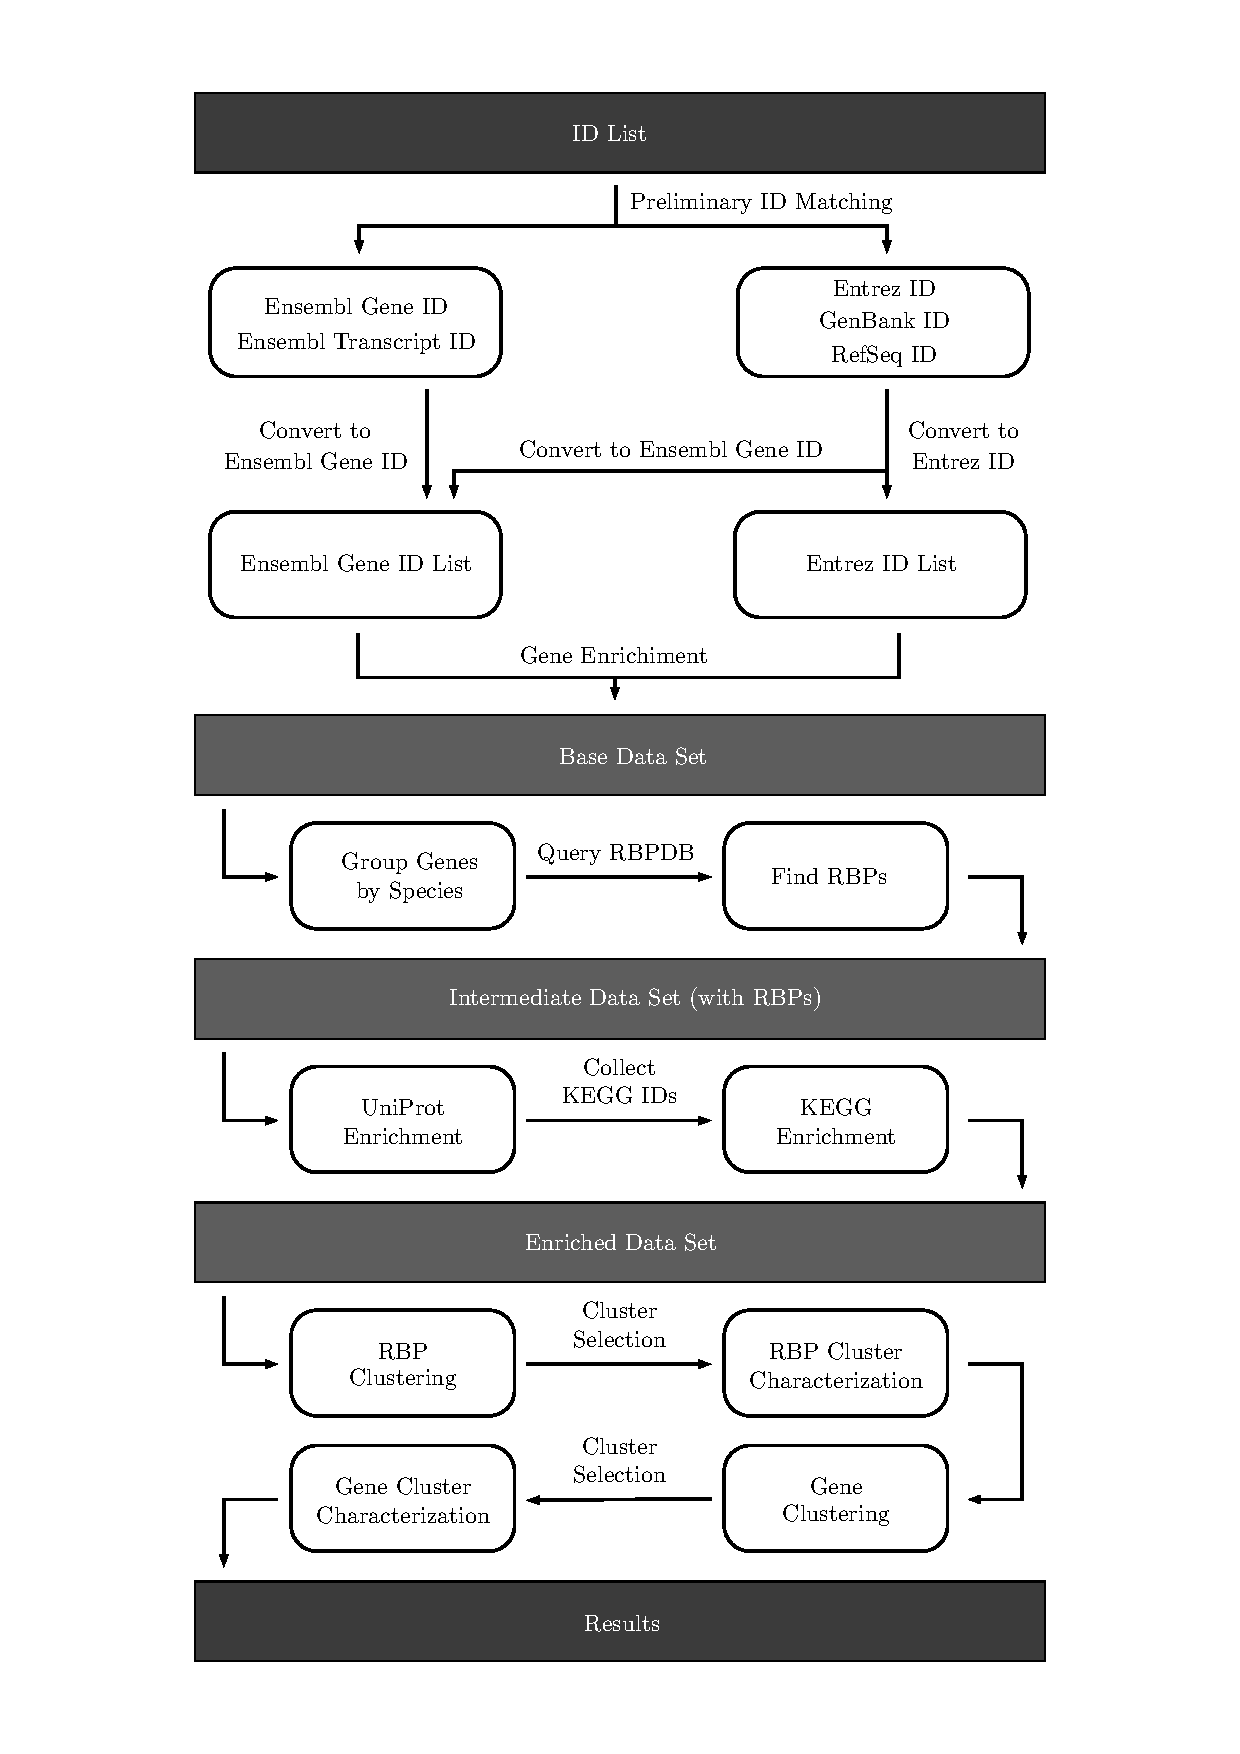
\includegraphics[width=0.73\textwidth]{workflow}
    \caption[PBS Finder workflow]{
      PBS Finder workflow. Note that error paths were not represented for
      simplicity. However, every component implements health checks, that may
      stop the entire analysis if the minimum requirements for success are not
      met.
    }
    \label{fig:workflow}
  \end{center}
\end{figure}

\subsection{Base Analysis}

The first step in the pipeline is to prepare the gene identifiers for the
following analysis steps. These identifiers can be written in five different
notations, as described in Section \ref{sec:descworkflow}. As such, identifiers
are separated according to their automatically detected notation in those five
groups. However, some of those identifiers may be invalid, despite appearing to
fit in one of the possible notations. It is assumed that if an identifier is
valid, it can at least be converted to either \emph{Ensembl Gene} or
\emph{Entrez} notation. These notations were chosen because they are the native
notations for genes in the used platforms (Ensembl and NCBI). This conversion is
done using bioDBnet's \cite{Mudunuri15022009} identifier conversion service. The
service was chosen for its simplicity and its large conversion database, that
draws from multiple conversion services like NCBI or Ensembl. \emph{Entrez}
conversion is only attempted if \emph{Ensembl Gene} conversion is not available.
While none of those platforms are preferred, converting as many identifiers as
possible to one convention helps to maintain data set coherence.

Since only two lists remain, one with \emph{Ensembl Gene} identifiers and the
other with \emph{Entrez} identifiers, information about those genes' transcripts
must be collected. This information includes the transcript's name, its
identifier, and its relevant genetic sequences. This information is collected
using their corresponding platform (Ensembl or NCBI).

The transcript sequences are then used to retrieve the related RBPs using RBPDB,
an online RNA binding protein database \cite{Cook01012011}. For each sequence
RBPDB finds every possible RBP, along with its name, location and binding
sequence. A complete list of all information retrieved for both genes and
transcripts can be found in Table \ref{tab:info_gene}. For a specific
transcript, if the retrieved 3’ UTR sequence is at least three hundred base
pairs long it will be used with RBPDB. If the 3’ UTR is too short, the 3’ UTR
downstream sequence (genomic sequence) will be used, with a fixed length of one
thousand base pairs. If none of the above situations is possible, the 3’ UTR
will be used as is (if it is at least one base pair long). Note that while the
5' UTR sequence is also collected (when available), the consulted experts were
interested in analysing only the 3' region. This information is sufficient to
answer one of this thesis' problems. However, it will be enriched and further
analysed, bringing greater benefits to researchers.

\begin{table}[!htb]
  \centering
  \begin{tabular}{{l} | {l}}
    \multirow{3}{*}{\textbf{\emph{Gene}}}
    & Transcript identifiers\\
    & Gene name*\\
    & Species*\\ \hline
    \multirow{3}{*}{\textbf{\emph{Transcript}}}
    & Protein identifiers\\
    & Transcript name*\\
    & Genetic sequences (3' UTR, 3' UTR downstream, 5' UTR)\\
    & Names, locations and bind sequences of RBPs\\
  \end{tabular}

  \caption[Information retrieved for genes and transcripts in the base analysis stage]{
    Information retrieved for genes and transcripts in the base analysis stage.
    Information marked with \qt{*} represent optional information; it might be
    relevant to the researcher and is therefore shown if available, but it is
    not crucial to the analysis. On the other hand, the unmarked fields
    represent required information, without which analysis on that particular
    gene/transcript cannot continue.
  }
  \label{tab:info_gene}
\end{table}

\subsection{Data Set Enrichment}

Given the RBP names obtained in the base analysis stage, a query is made to
UniProt in order to obtain their respective accession identifiers. These are
used internally by UniProt to refer to specific proteins. With the accession
identifiers, the pages for each RBPs can be retrieved and analyzed individually.
These pages contain information about their respective RBPs, including keywords,
related tissues and information about the protein's ontologies (cellular
components, molecular functions and biological processes).

The information collected from UniProt may also contains links to the KEGG web
platform. Among other useful information, KEGG contains information about
protein pathways. A pathway is a sequence of actions, related to specific
molecules, that produce certain changes within a cell, when performed. This
information is crucial to understand the function of RBPs. As such, it is
collected for further analysis (see Table \ref{tab:info_prot} for a complete
list of all information retrieved).

The first step for this phase is to use the protein names to retrieve a list of
matching \emph{UniProt Accession} identifiers. By default PBS Finder will try to
find a reviewed accession whose species matches the species in question. If this
is not possible it will fallback to an unreviewed accession, from the same
species. In case this is also not possible, it will try to find a reviewed human
analogue accession or, as a last case, an unreviewed one. After finding the
identifiers, the batch retrieval service is used to enrich the protein
information. This information includes ontologies, related tissues, and
references to external databases. From these references, KEGG identifiers in
particular are used to retrieve information about pathways in which the RBPs are
expressed. For each pathway, both its name and link to the KEGG pathway viewer
are provided.

\begin{table}[!htb]
  \centering
  \begin{tabular}{{l} | {l}}
    \multirow{8}{*}{\textbf{\emph{Protein}}}
    & Protein name\\
    & UniProt identifier\\
    & Accession species\\
    & Related tissues*\\
    & Keywords*\\
    & Pathways*\\
    & Ontologies*\\
    & URLs to external platforms*\\
  \end{tabular}

  \caption[Information retrieved for proteins in the data set enrichment stage]{
    Information retrieved for proteins in the data set enrichment stage.
    Information marked with \qt{*} represent optional information; it might be
    relevant to the researcher and is therefore shown if available, but it is
    not crucial to the analysis. On the other hand, the unmarked fields
    represent required information, without which analysis on that particular
    protein cannot continue.
  }
  \label{tab:info_prot}
\end{table}

\subsection{Clustering Analysis}

The last stage of the workflow is clustering analysis. Two different types of
clustering approaches were conceived: \emph{clustering by RBP presence} and
\emph{clustering by RBP information}. Note that this analysis will not be
performed if the quantity of available data is below certain thresholds
(typically the tool will not analyse data sets that have less than ten genes
and/or ten RBPs).

\subsubsection*{Clustering by RBP Presence}

In the first case, the clustering analysis is only conducted at the gene level.
Two genes are similar if they are associated with the same RBPs. Inversely, two
genes that do not have any (or few) RBPs in common are considered \qt{distant}. The
tool makes an additional step in order to determine which RBPs are common in one
particular group, while being absent in all the other groups. This information
allows researchers to easily determine which RBPs can be used to interact with a
particular group of genes, while not affecting the others.

\subsubsection*{Clustering by RBP Information}

In the second case the clustering process has two phases. In the first phase
RBPs are grouped based on their similarity. Similarity is computed using a set
of attributes that include (depending on availability): pathways; tissues where
the RBP is expressed; keywords describing their main functions; and other
relevant information such as ontologies (biological processes, molecular
function and cellular components). The tool compiles a list of defining features
for each group (to later present to the user). However, in this case the RBP
groups will be used to group similar genes. Unlike the previous method,
similarity between genes is not only measured in how many RBPs they have in
common. In this case any two genes may be considered similar if both are related
to RBPs that were grouped together in the previous step, even if they do not
share exactly the same RBPs between them.

\subsubsection*{Setup Variation}

To produce the final results multiple clustering experiments are attempted. Due
to the small amount of time that the chosen clustering algorithms need to run it
is possible to execute a large number of attempts and then choose only the best
results. Each attempt is a variation of the analysis parameters, being that each
possible value for a parameter is combined with every value for the remaining
parameters, giving rise to a large number of experiments. When clustering by RBP
presence the variable parameters are: clustering algorithm (either hierarchical
clustering or partitioning around medoids); and the number of clusters (between
two and ten). While clustering by RBP information the same variable attributes
apply. However, the decision about what RBP information is used for their
comparison is also variable, from a minimum of two information fields. For
example, in a particular clustering attempt only information about the RBPs'
pathways and related tissues may be used, while another attempt may use all
available information. Furthermore, for this particular type of analysis the
representation of the data set can also vary. The data set can be represented
either as a binary matrix (as is the case in clustering by RBP presence) or by a
Jaccard distance matrix, calculated from the sets of possible values for each of
the protein's attributes.

\subsubsection*{Result Selection}

With the large number of results obtained from all the clustering attempts, it
is not reasonable to expect a user to manually choose the ones that are most
interesting. As such, internal evaluation techniques for clustering are coupled
with rules that define minimum acceptance criteria for results, narrowing the
result space to only one for each type of clustering. Algorithm
\ref{algo:secsel} represents the method used for result selection.

\begin{algorithm}
  sort clustering results by average silhouette (descending)\;
  filter clustering results with clusters with less than 8\% of data set objects\;
  \emph{abundance\_frequency} = 0.90\;
  \While{abundance\_frequency $\geq$ 0.50}{
    \ForEach{clustering result}{
      classify as abundant any attribute with frequency $\geq$ \emph{abundance\_frequency}\;
      remove abundant attributes that appear in multiple clusters\;
      \uIf{at least one unique abundant attribute exists for each cluster}{
        select cluster\;
        break loop\;
      }
      \Else{
        \emph{abundance\_frequency} = \emph{abundance\_frequency} $-\ 0.05$\;
      }
    }
  }
  \uIf{a cluster was selected} {
    return selected cluster\;
  }
  \Else{
    return cluster with highest average silhouette\;
  }

  \caption[Selection of best clustering results]{
    Selection of best clustering results.
  }
  \label{algo:secsel}
\end{algorithm}

\subsubsection*{ILP Clustering}

Clustering using ILP techniques was also attempted. The main objective of this
approach was to uncover more information about the implicit relationships
present in the data sets. While conventional clustering methods present only the
data set objects grouped in clusters, with ILP it is possible to understand
exactly what rules were used to form those clusters.

The devised approach had two steps. First, the results for each new job would be
represented in the form of Prolog clauses. Second, those clauses would be used
as data set for the ERDA \cite{fonseca2012conceptual} clustering system, running
on top of YAP Prolog \cite{citeulike:8884858}. However, due to problems with the
available tools, this approach could not be included in the current version of
PBS Finder.

\subsection{Web Interface}

%\begin{Notes}
%- Talk about all information available in each view.\\
%- Talk about the types of results to export.\\
%- Talk about GridFS, and the need of pre generate results files to minimize long
%loading times.\\
%\end{Notes}

\subsubsection*{Job View}

Job view, also known as main view, is the default projection of a job's results
(Figure \ref{fig:job_view}). It gives the user a matrix that matches every gene
(and transcript) in the data set with their corresponding binding proteins, as
well as an histogram of the genes (a bar chart of the number of genes with which
each RBP binds). This matrix also contains two columns that provide information
about how the genes were grouped, based on the two distinct clustering
techniques. In addition to this information, clicking any group of genes will
give the user a list of all the characteristics that differentiate that
particular group from all the others.

This view also contains a mechanism that allows users to provide feedback and
report problems. Clicking the \qt{Report a problem} button the user is presented
with a form that allows them to provide a brief description of the problem. If
the user chooses to send that report, the web platform will send an email to its
administrator, containing the submitting user's information, the problem
description and a direct link to the offending page.

\begin{figure}[!htb]
  \begin{center}
    \leavevmode
    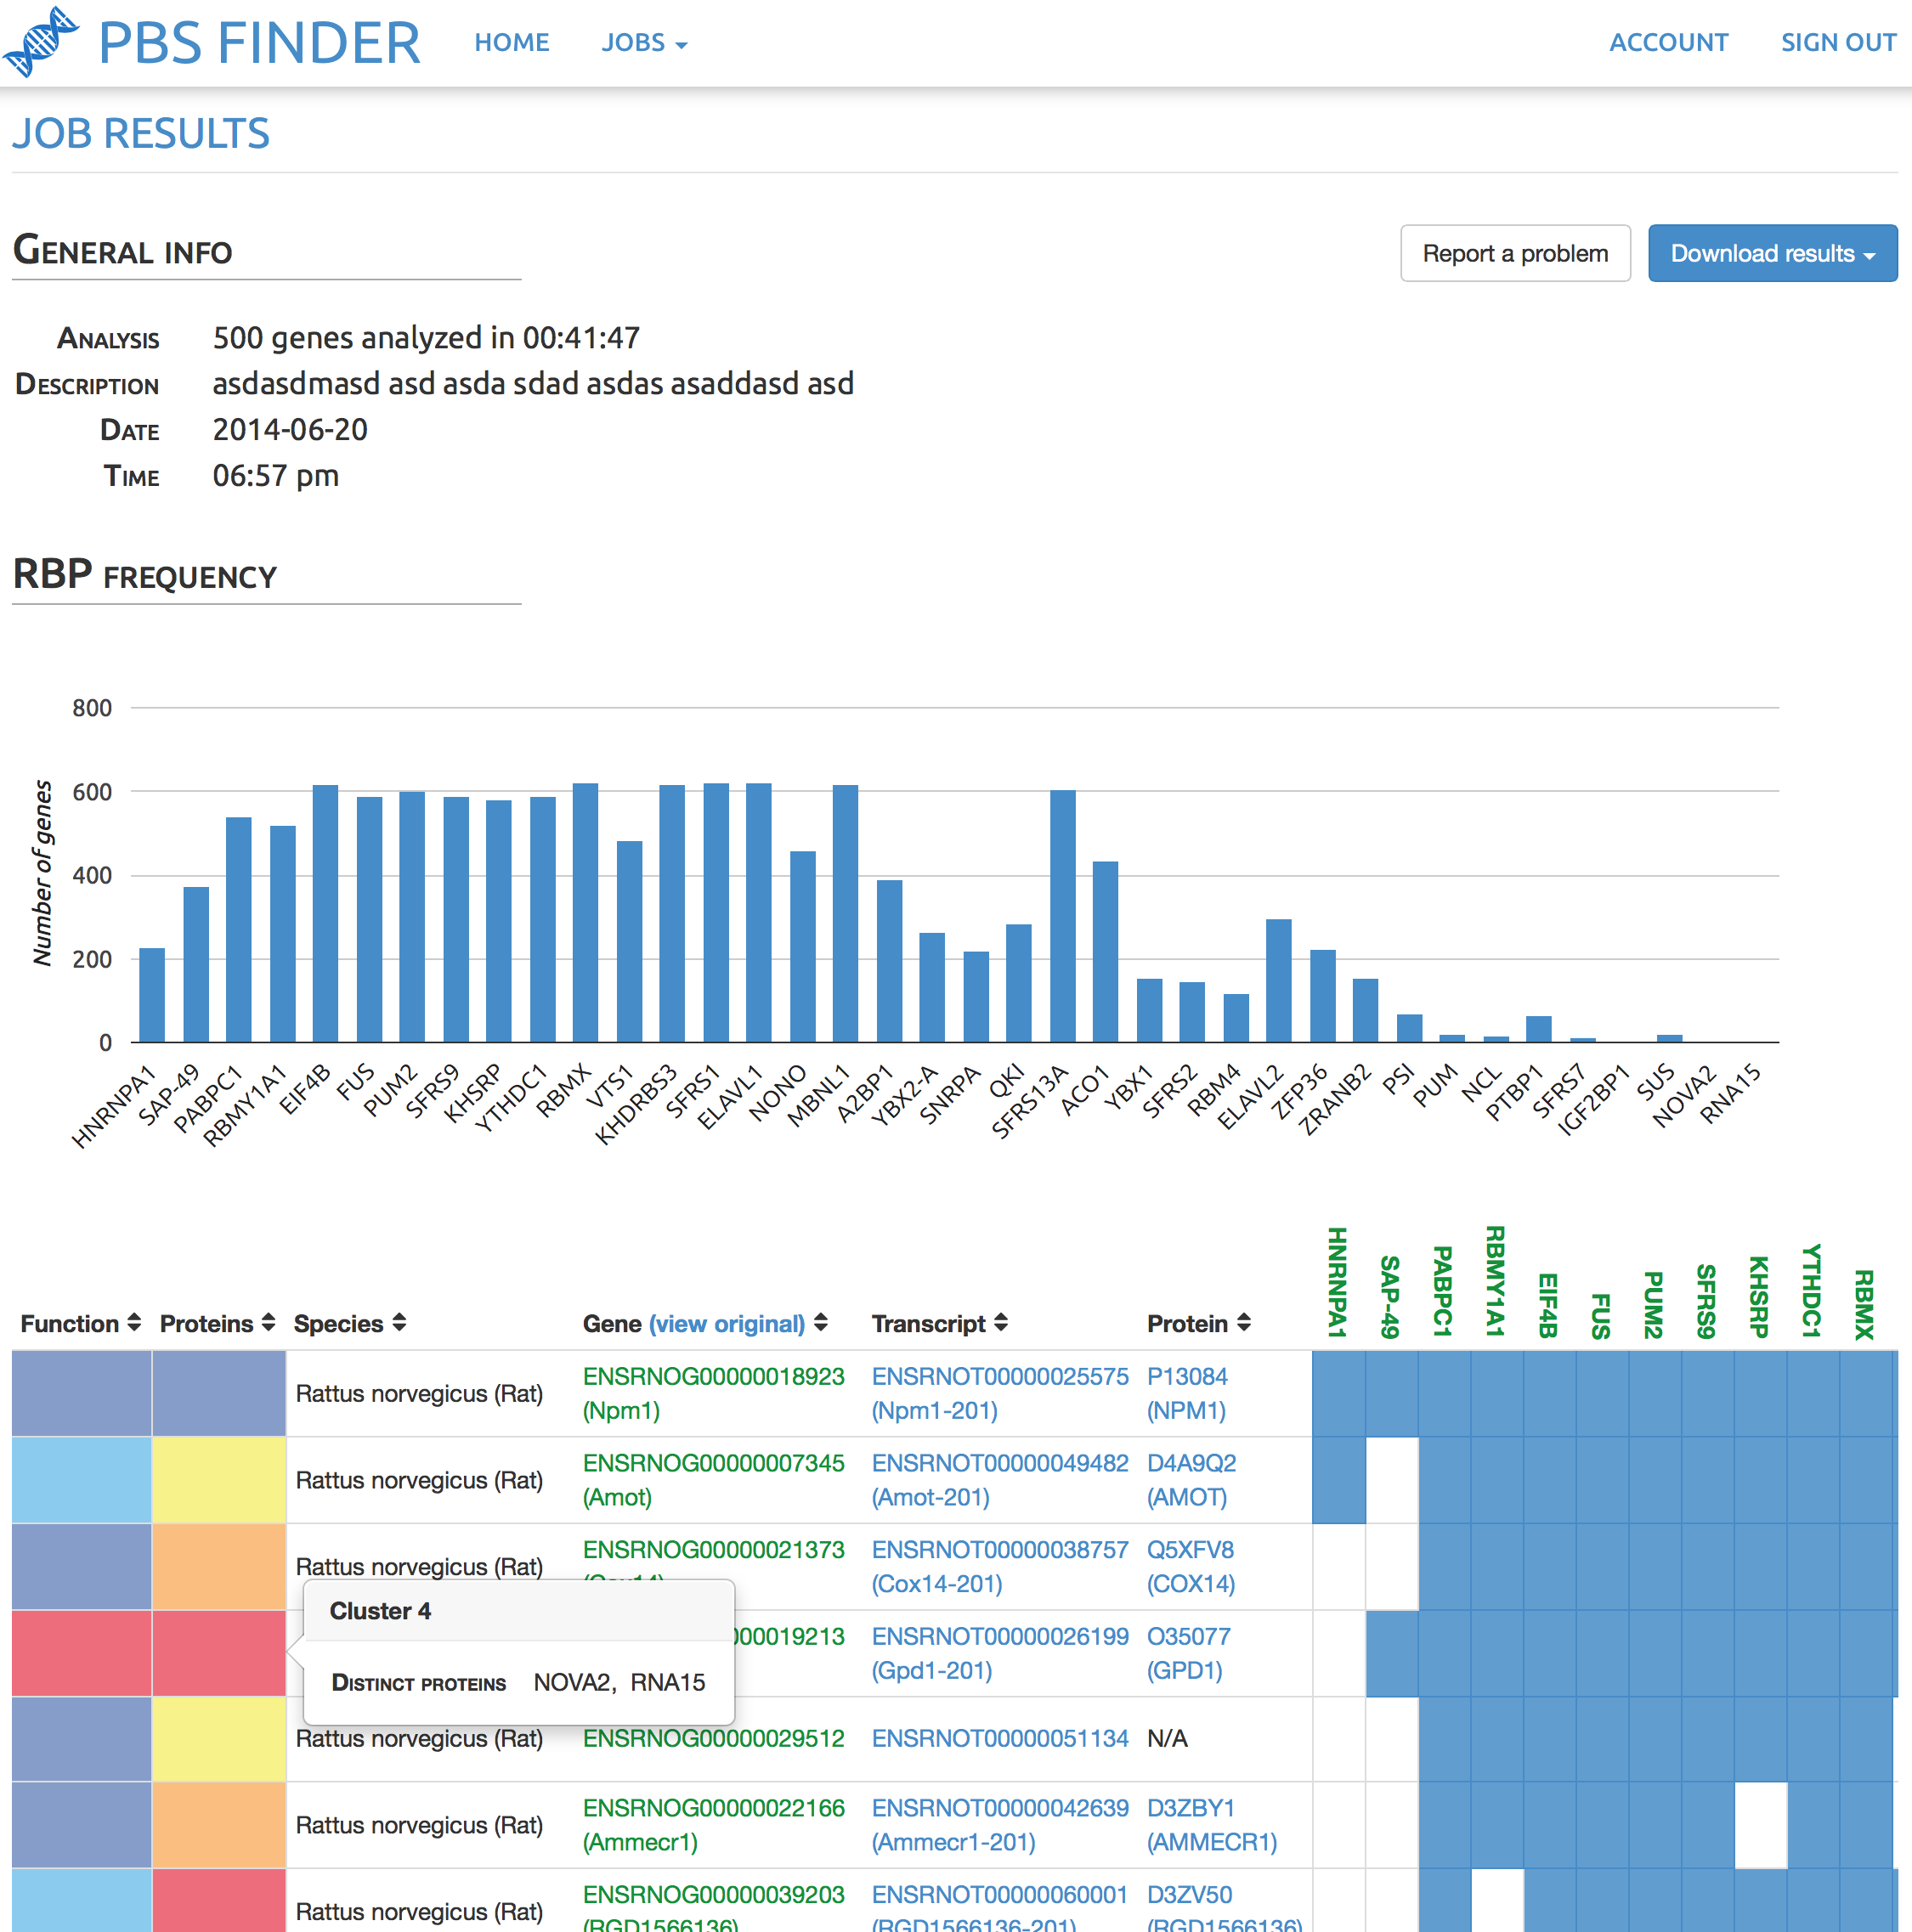
\includegraphics[width=\textwidth]{job_view}
    \caption[Job view example]{
      Job view example, also known as main view. It is comprised by three main
      components: general information (which includes data download); RBP
      frequency histogram; and RNA binding protein matching table.
    }
    \label{fig:job_view}
  \end{center}
\end{figure}

\subsubsection*{Transcript View}

The transcript view (Figure \ref{fig:trans_view}) offers more detailed
information about the transcript's binding proteins, giving for each protein the
base pairs that compose the binding site (and its start and stop positions) and
a percentage score of the match's quality. A maximum of three different genetic
sequences (5’ UTR, 3’ UTR and 3’ UTR downstream\footnote{5' UTR and 3' UTR are
non-coding regions located before the initiation codon and after the termination
codon, respectively. While these regions are not translated to useful genetic
products, their presence is important to regulate cellular processes.}) are also
displayed, depending on their availability. Whenever possible, related links to
other platforms are presented (Ensembl, NCBI and UniProt). Like the job view, it
also contains clustering information, but in this case only one column, that
shows how the RBPs related to that specific transcript were grouped. Also
similarly to the job view, users can click any group to obtain relevant
information about the defining characteristics of that particular group.

\begin{figure}[!htb]
  \begin{center}
    \leavevmode
    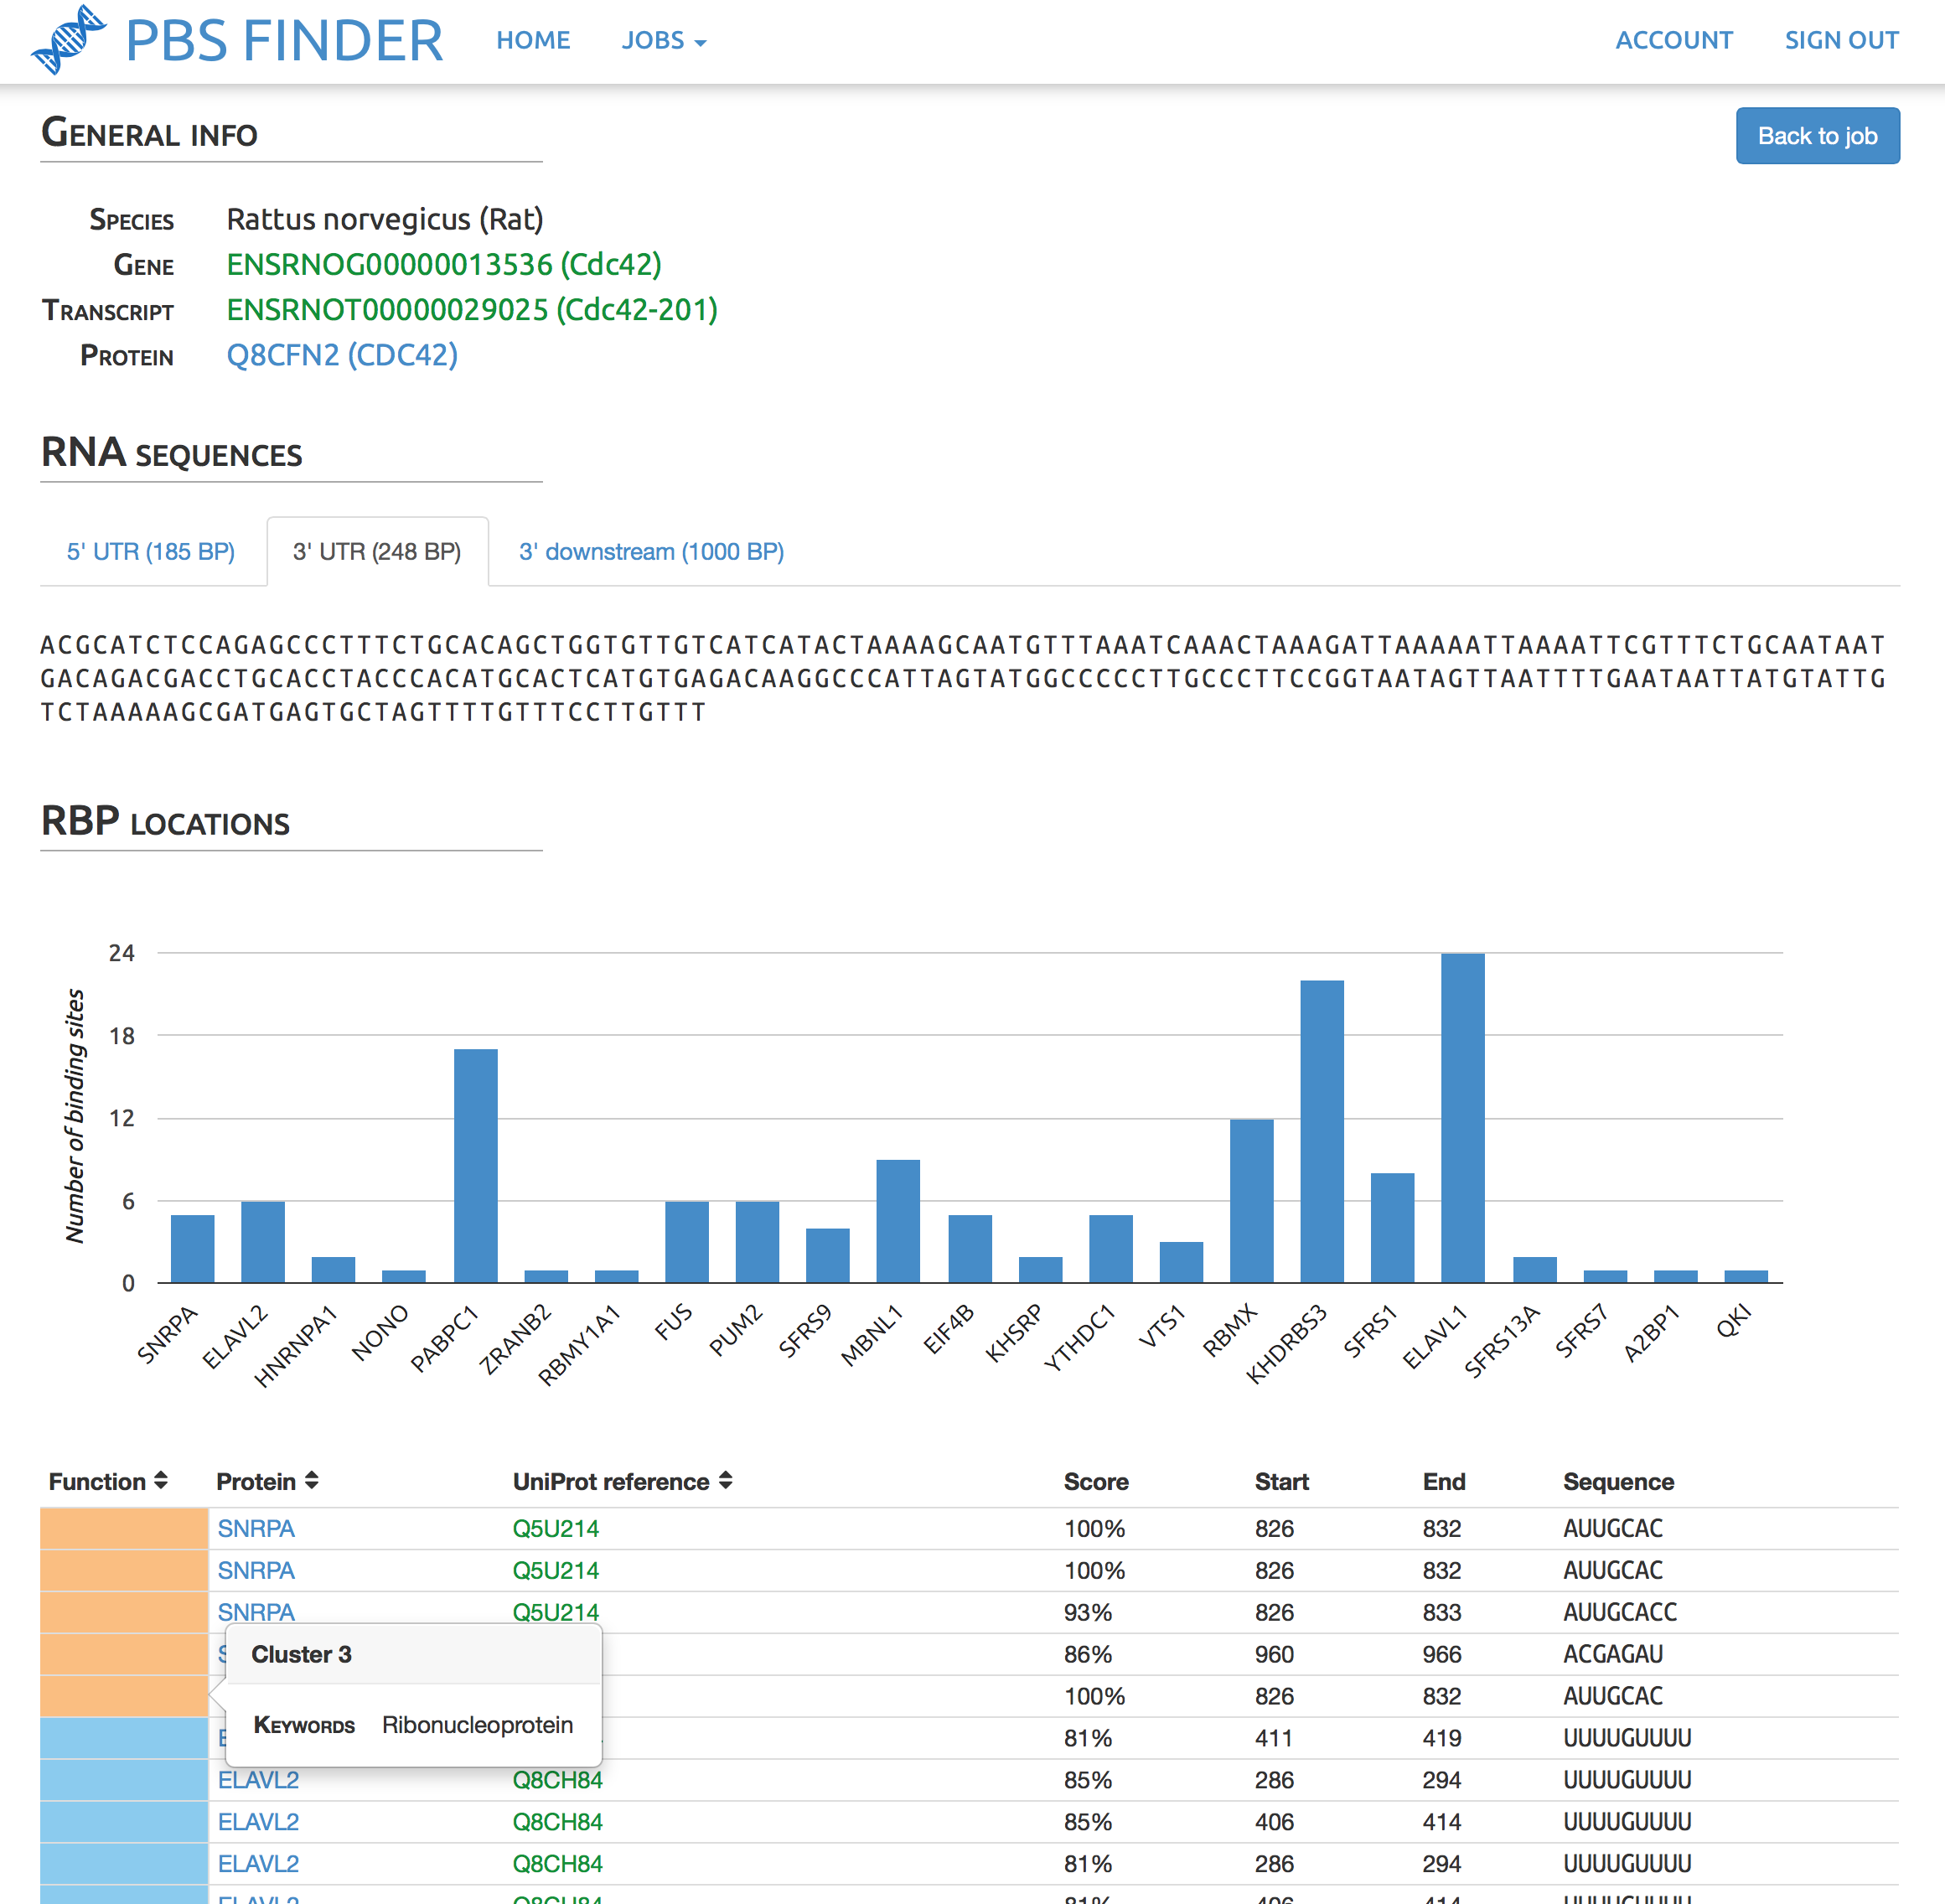
\includegraphics[width=\textwidth]{trans_view}
    \caption[Transcript view example]{
      Transcript view example. It contains four main areas: general information
      about the transcript; RNA sequences (5’UTR, 3’UTR and 3’UTR downstream are
      shown depending on availability); RBP locations histogram; and RBP
      location table (including clustering results and match sequences).
    }
    \label{fig:trans_view}
  \end{center}
\end{figure}

\subsubsection*{Protein View}

The protein view (Figure \ref{fig:prot_view}) displays relevant classification
information for every RBP (when available). This information includes the
protein's name, links to other platforms (UniProt, KEGG, Gene3D, etc.), tissues
in which the protein might be expressed, the protein's ontologies and the pathways
in which the protein participates. Each pathway is coupled with a link to the
corresponding KEGG pathway browser page.

\begin{figure}[!htb]
  \begin{center}
    \leavevmode
    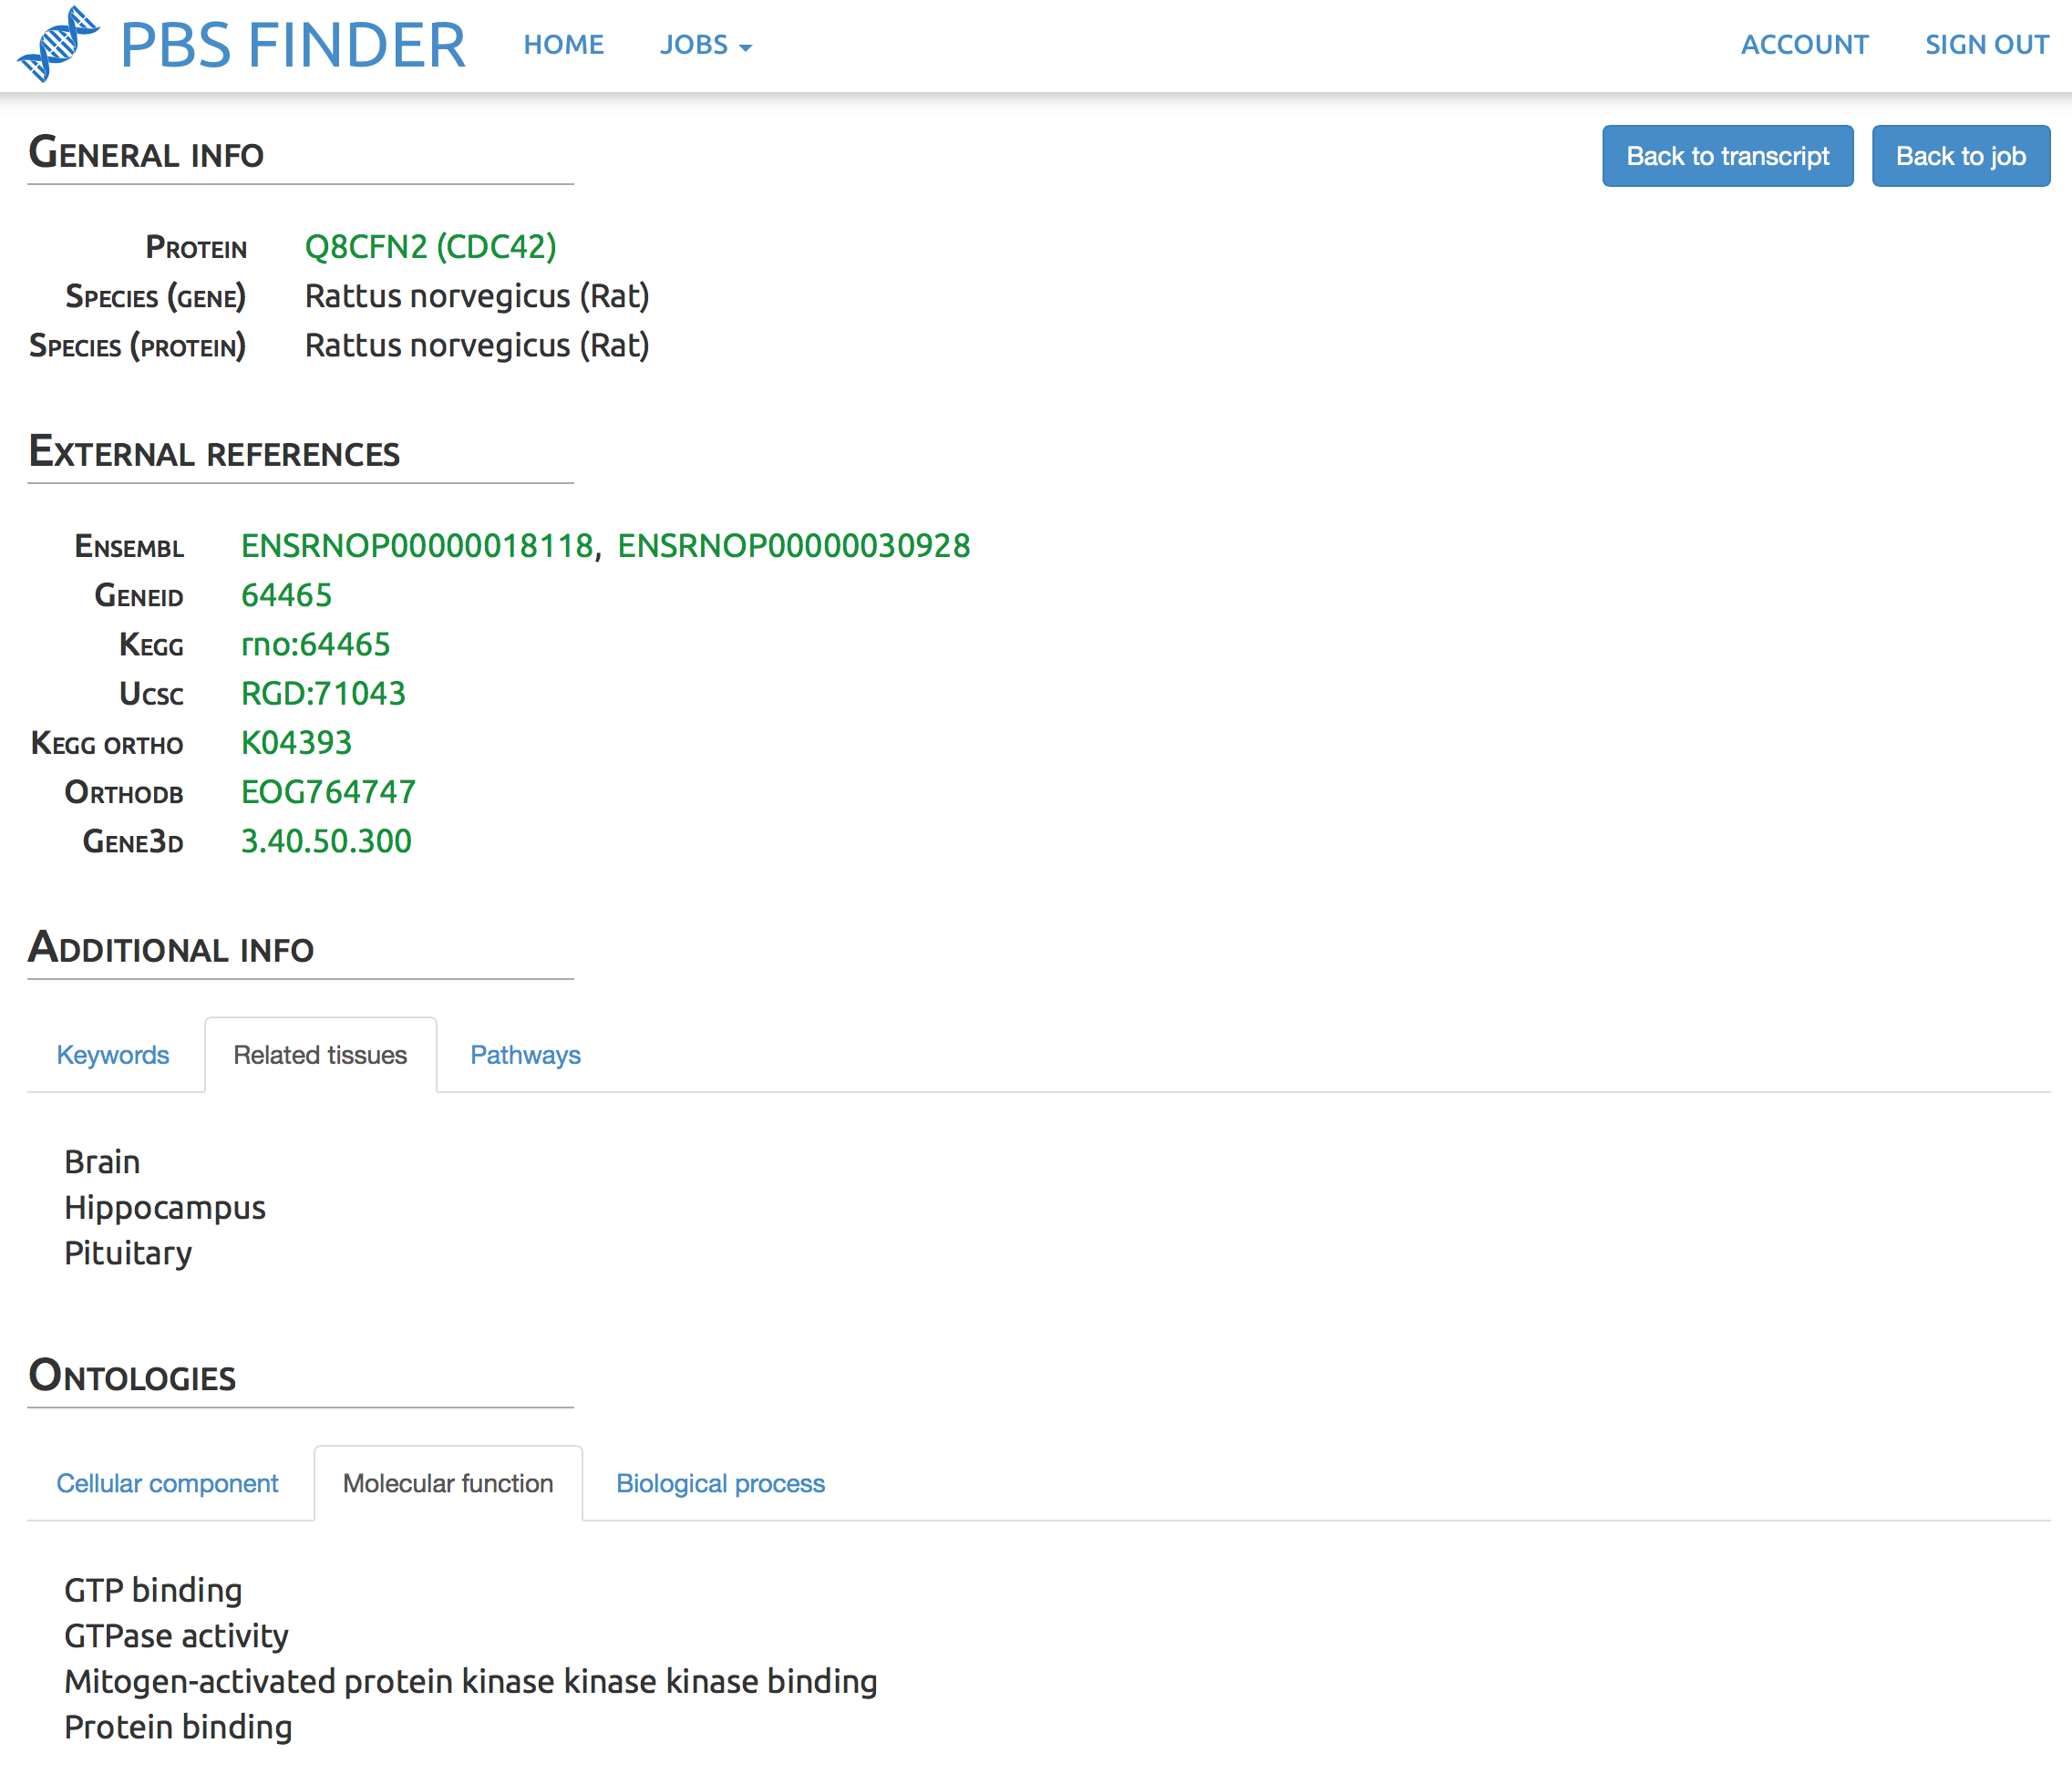
\includegraphics[width=\textwidth]{prot_view}
    \caption[Protein view example]{
      Protein view example, containing four relevant areas: general information
      about the protein; links to other web platforms with relevant information
      about the protein (note that some of those platforms might not contain
      information about a particular protein, and therefore no links can be
      shown); additional info, including keywords, related tissues and pathways
      in which the protein is expressed; and lastly, information about the
      protein's ontologies, including cellular components, molecular functions
      and biological processes.
    }
    \label{fig:prot_view}
  \end{center}
\end{figure}

\subsubsection*{Exporting the Results}

Besides browsing, users can download their results as text files. Three
different types of data projections of the results are provided: \emph{RBP
data}, \emph{protein data} and the \emph{complete data set}. RBP data can be
downloaded in either comma-separated values (CSV) or tab-separated values (TSV)
format. This file gives the user a match matrix of binding proteins, similar to
the one in the job results view, as well as species, gene and transcript
information. Protein data can also be downloaded in both CSV and TSV formats. It
gives a more complete view of the results, including species, gene, transcript
and protein identifiers and additional protein information (keywords, related
tissues, ontologies, etc.). Finally, the data set may be downloaded as a
complete Prolog predicate representation of the job results. This is the same
representation of the results that was created with the usage of ILP clustering
techniques in mind. While it was not possible to use those techniques, the
produced data set representation might still be of use to researchers.

While in most cases these data representation conversions are apparently
instantaneous, for large data sets they may take an additional amount of time.
This would cause the web application to seemingly block if the user tried to
download one of those files. To solve this problem all files are generated
during the analysis process, then stored in the web application's MongoDB
instance through GridFS\footnote{GridFS is a functionality integrated in MongoDB
that allows a simple file system to be simulated inside a database. Files are
divided into small chunks and those chunks are stored as regular MongoDB
documents.}. This allows those files to be downloaded instantly, as they need
only to be generated once.

%\section{Deployment}

%\begin{Notes}
%- Talk about tested deployment platforms.\\
%- Talk about system requirements.\\
%\end{Notes}

\section{Chapter Conclusions}

%\begin{Notes}
%- Generic chapter conclusion.\\
%\end{Notes}

In this chapter we presented a concrete approach to the development of the
proposed solutions. We reviewed their most important features and implementation
choices. Further examples of their usage is available through a case study in
Chapter \ref{chap:casestudy}.
